\chapter{Results}
\label{cha:results}


This chapter discusses the basic findings of the analysis of the proposed peer influence model.
All results were obtained from synthetic networks, with a fixed size of \( n = 5,000 \) nodes, which were generated over \( T = 75,000 \) iterations.
The here presented properties of the time-varying networks were obtained by averaging the results of 40 independent runs, which is necessary due to the stochastic nature of the model.
The model parameter responsible for the formation of the community structures are set to \( p_{\Delta} = 0.90 \) for the triadic closure probability, \( \delta = 1 \) for the link reinforcement constant, and \( p_{d} = \num{5e-05} \) for the node deletion probability for every experiment.
Furthermore, the critical peer influence threshold was fixed to \( \theta = 0.10 \).
This reflects the idea that only a relatively small number of active neighbors is sufficient to increase the activity of a node in a significant way.

The time-dependent topological properties of the integrated network, which are discussed in \cref{sec:integrated-network-properties}, are measured only for nodes that are part of the temporal network.
This means that nodes, which were removed earlier due to the node deletion process do not influence the properties of the integrated network any more.
\Cref{sec:network-activity} contains an overview of the overall network activity with respect to different levels of peer influence.
The effect of the peer influence mechanism on the inter-event time distribution in the network is examined in \cref{sec:inter-event-time-dists}.
Furthermore, the distributions of the node degrees and tie strengths (i.e., the link weights) derived from the integrated networks are the subject of \cref{sec:weight-and-degree-distribution}.
All these experiments are performed for different values for the maximum peer influence probability \( q \).
However, the analysis performed in the last section of this chapter (\cref{sec:softmax-rescaling}) uses a fixed value for the peer influence level and discusses how different values for \( \beta \), the inverse temperature for the softmax weight rescaling, changes the peer influence effects in the network.
The temporal networks, which are used in the experiments of the first four sections of this chapter, adopt the current average tie strength as temperature for the softmax weight rescaling.
Therefore, \( \beta \) is set to the to the reciprocal value of average weight in the integrated network in each iteration after the first one (i.e., \( \beta = 1 \) in the initial round to avoid division by zero, since no ties have been formed yet).


%% ========================================================================
%% ========================================================================


\section{Time-dependent Integrated Network Properties}
\label{sec:integrated-network-properties}

Not only the final integrated network of all 75,000 instantaneous networks and its properties are of great interest, but also how they evolve during the simulation.
This allows to get a deeper understanding on how the model shapes the community structures in the network and the effects of the peer influence mechanism on it.
The integrated network is build in an iterative fashion to make these observations possible.
A snapshot of the integrated network is taken after the newly formed ties are included and the weights of already established links are updated in every time step.
Features like the average local clustering coefficient or the average weight of the ties are calculated for each of the 75,000 integrated network snapshots.
This allows to examine how the topology and other measures change over time.

The first, and most interesting, measure that can be investigated in this way is the average local clustering coefficient \( C(t) \).
\Cref{fig:avg-local-cc-full} depicts the development of it over the course of the simulation for different levels of peer influence.
The graph of this function has a very distinctive pattern, which was already explained in the original work by \citet{Laurent2015}.
The average clustering coefficient is very small in the first few hundred iterations, due to the sparsity of the integrated network.
Almost all nodes are disconnected and the number of triangles, which have already formed is relatively small compared to the size of the network.
However, \cref{fig:avg-local-cc-full} also shows that the clustering coefficient grows very fast until it reaches its maximum value after a short period of time.
This rapid increase is caused by the cyclic closure mechanism of the model.
Nodes that become active in this early stage first have to introduce some ties with nodes which are selected using the focal closure mechanism.
This does not increase the average local clustering coefficient in a significant way, however, it establishes the egocentric networks.
After the first triangles are closed, the first strong ties start to develop.
These emerging strong ties amplify the biased local search of the triadic closure mechanism and result, on one hand, in more triangles, and on the other hand, in the reinforcement of already established triangles and the associated strong ties.
This leads to a high local clustering in the established communities.
However, weak ties are eventually also introduced to the network, due to the focal closure mechanism.
They are rarely involved in the formation of new triangles, due to the bias towards strong ties, which contributes to the decrease of the average local clustering coefficient until the network reaches its stationary state.


\myfig{avg-local-cc-full}
      {width=0.75\textwidth}
      {The average local clustering coefficient \( C \) as a function of time for different maximum peer influence probabilities \( q = 0, \, 0.01, \, 0.05, \, 0.1, \, 0.15\). }
      {Average local clustering coefficient as function of time}
      {fig:avg-local-cc-full}


The peer influence mechanism seems to influence the development of the local clustering in the beginning of the simulation significantly.
\Cref{fig:avg-local-cc-start} depicts the time-depended average local clustering coefficient in the initial phase of the simulation (i.e., for the first 10,000 iterations) for a range of possible values for \( q \).
It shows that the peak of \( C \) is reached faster for networks in which nodes are able to motivate their neighbors to some extend.
For instance, the network in which nodes are not able to influence their neighbors reaches it peak value for \( C \) after approximately 5,000 iterations, while the network with a maximum peer influence probability of \( q = 0.15 \) is more than 2,000 iterations faster.
However, the effect only occurs for networks with \( q > 0.05 \) and the actual maximum value of the local clustering coefficient only increases slightly for higher levels of peer influence (c.f. \cref{tbl:max-clustering} for the precise figures).
Furthermore, the proposed peer influence mechanism seems to have an positive effect on the development of the topological structures in the network by accelerating the process in the beginning.

The percentage of network activity, which is responsible for the reinforcement of ties in each iteration \( r(t) \) highlights this behavior as well.
In the beginning most activity is spend on the formation of new ties and therefore building the topological structures of the network, but after a while more and more activity is focused on reinforcing existing ties, which leads to a drastic increase of \( r(t) \).
This is also emphasized by the time required to reach the point from which on more than half of the total activity is spend on reinforcement.
This point is reached for the network with \( q = 0.15 \) after only 109 iterations.
The network with no peer influence takes with 229 iterations about twice as long, indicating that peer influence may play an important role in the first few iterations that shape the topology of the network.


\begin{figure}[htbp]
\centering
\begin{subfigure}[b]{0.485\textwidth}
  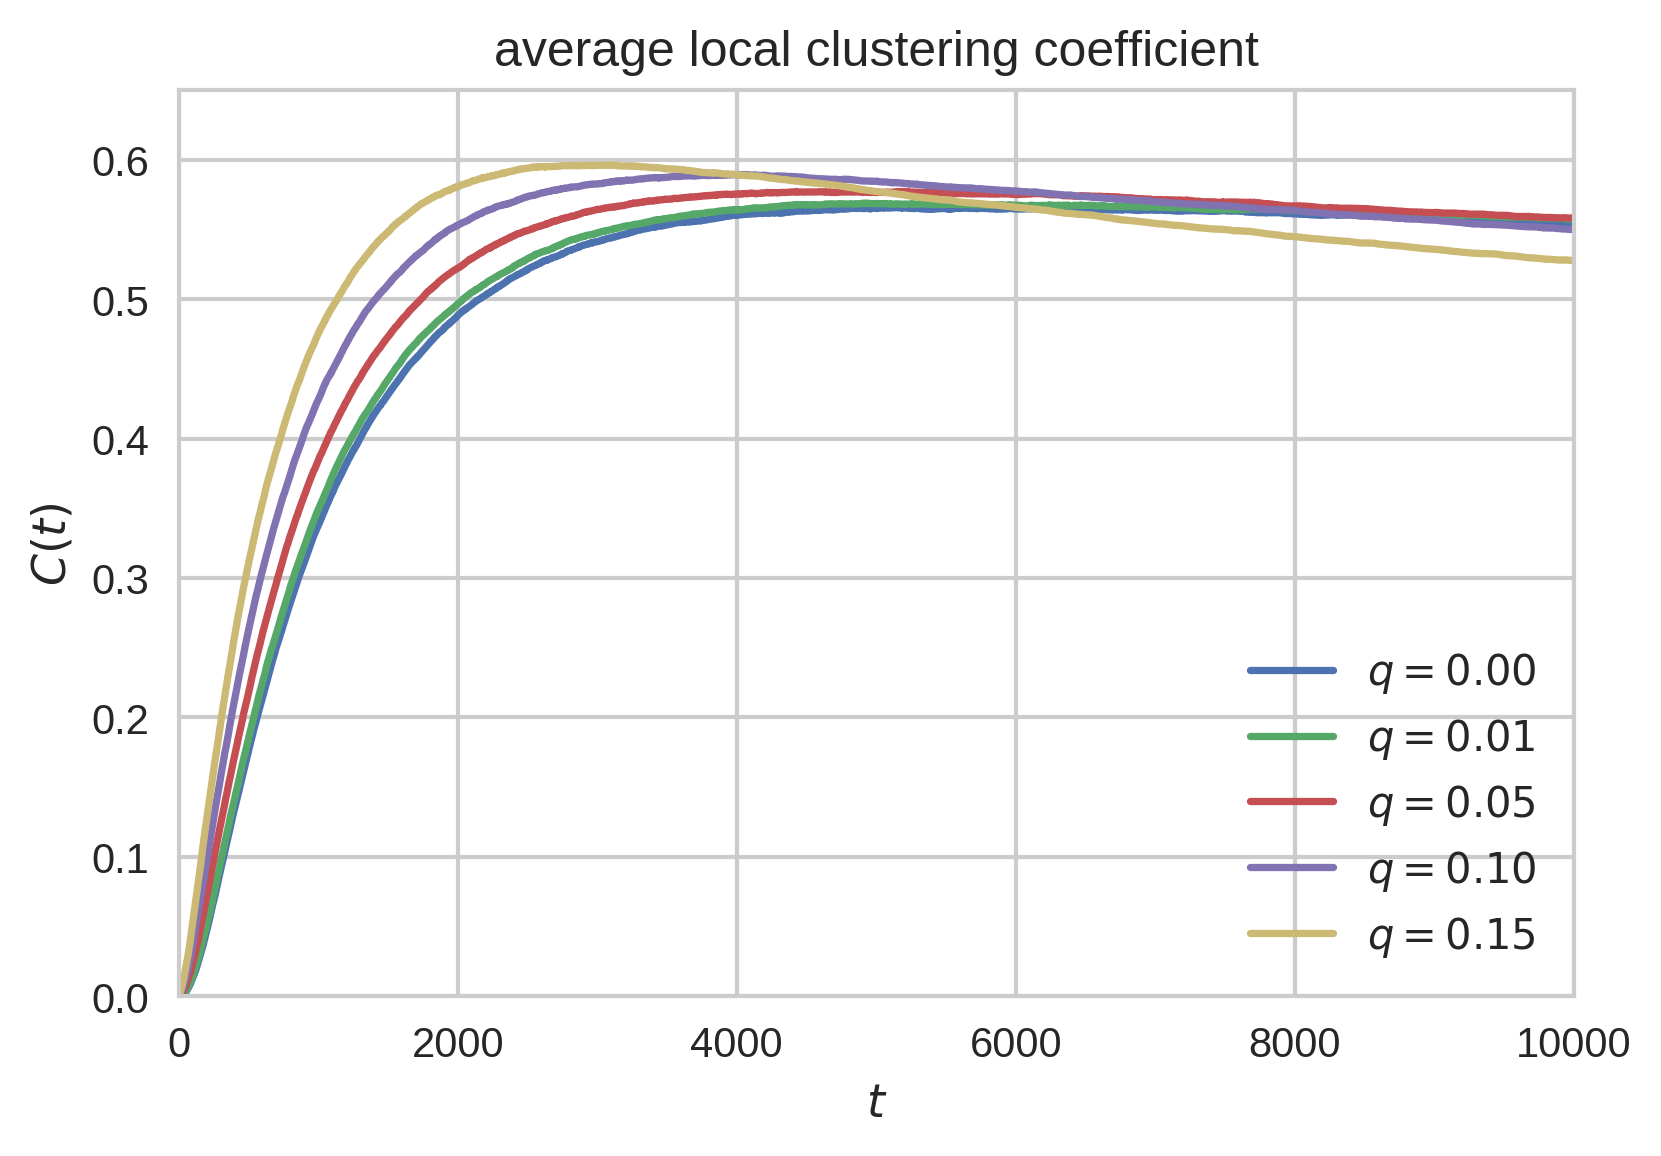
\includegraphics[width=\textwidth]{figures/avg-local-cc-start}
  \caption{}
  \label{fig:avg-local-cc-start}
\end{subfigure}
~
\begin{subfigure}[b]{0.485\textwidth}
  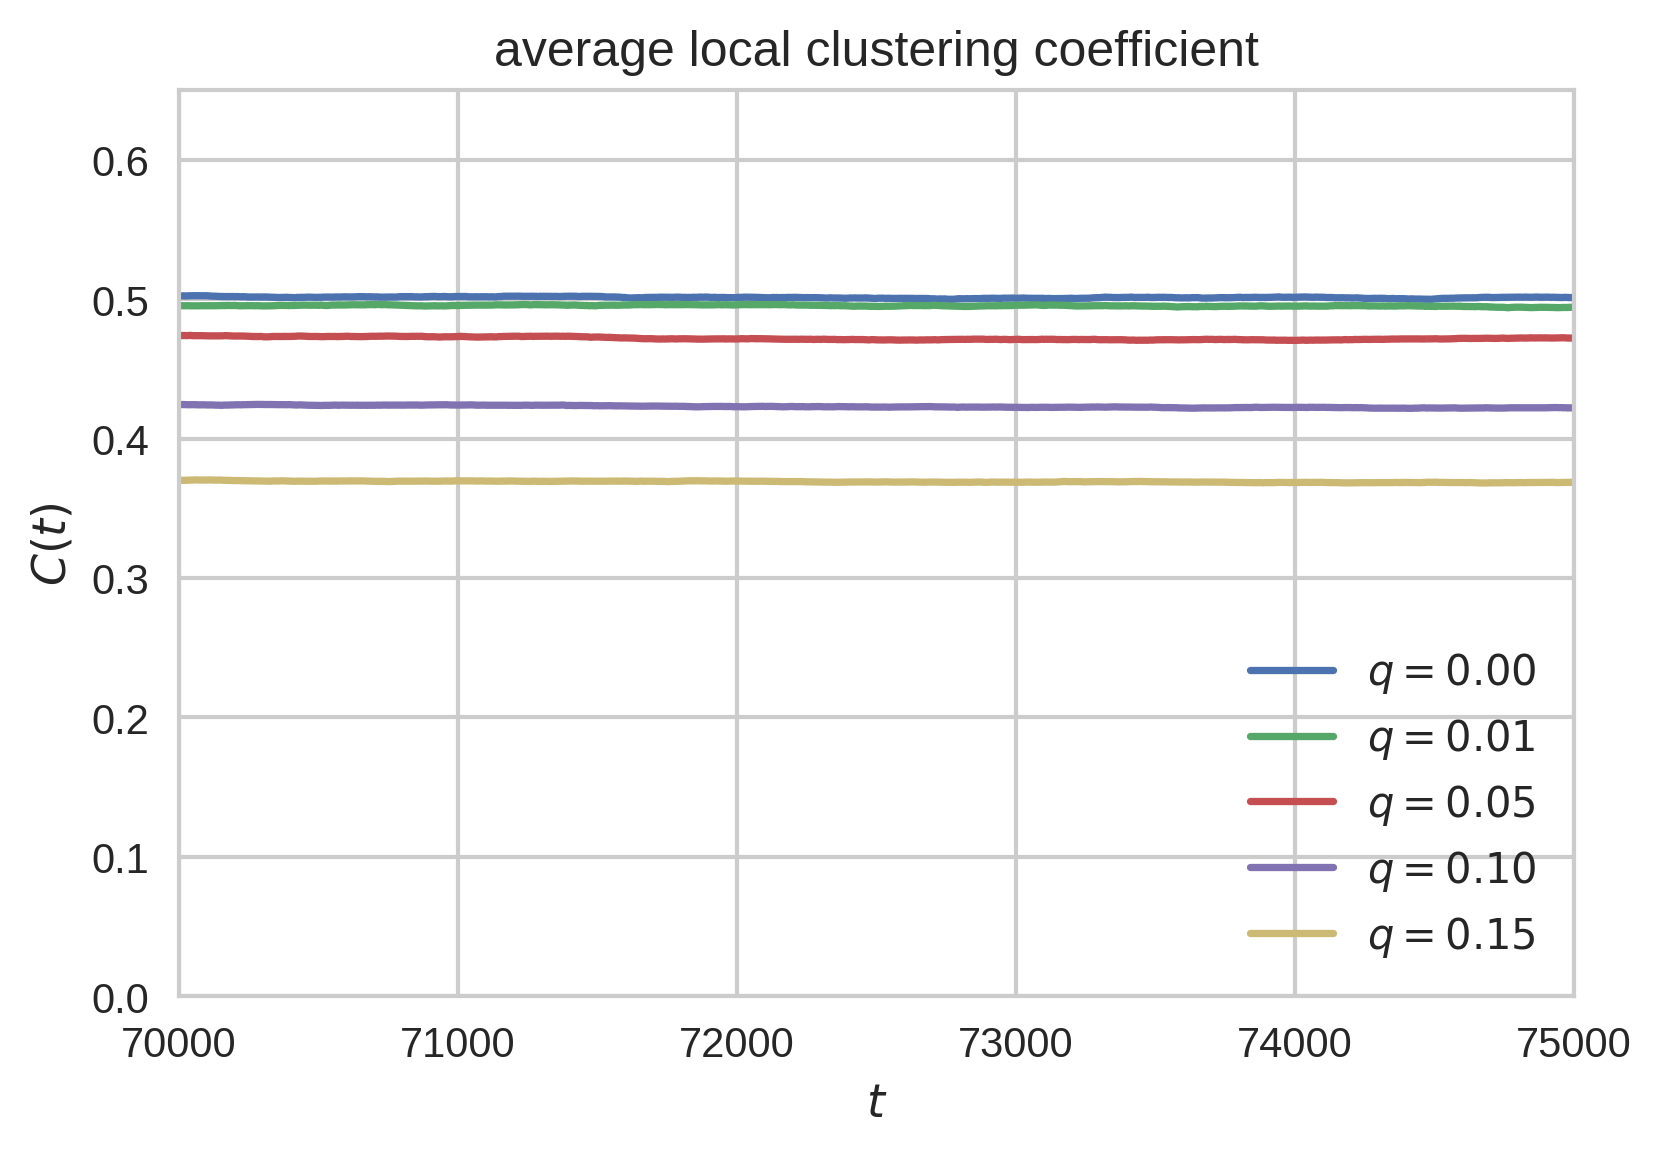
\includegraphics[width=\textwidth]{figures/avg-local-cc-end}
  \caption{}
\label{fig:avg-local-cc-end}
\end{subfigure}

\caption[Segments in the average local clustering coefficient evolution]{Segments in the evolution of the local clustering coefficient for different levels of peer influence. (\subref{fig:avg-local-cc-start}) shows the clustering coefficient for the first 10,000 iterations of the simulation, in which it reaches it maximum value and slowly starts to decrease. (\subref{fig:avg-local-cc-end}) depicts the stationary values for \( C \), which can be observed in the last 5,000 iterations.}
\label{fig:avg-local-cc-details}
\end{figure}


\begin{table}
\centering
\begin{tabular}{llllllll}
\( q \) & 0.00 & 0.01 & 0.025 & 0.05 & 0.075 & 0.10 & 0.15 \\ \hline
\( t_{\max} \) & 5,140 & 4,919 & 4,839 & 5,192 & 4,173 & 4,044 & 3,038 \\ \hline
\( C_{\max} \) & 0.5659 & 0.5689 & 0.5721 & 0.5773 & 0.5822 & 0.5895 & 0.5963
\end{tabular}

\caption[\( \max \) and \( \argmax \) of \( C(t) \)]{The maximum value for the local clustering coefficient \( C_{\max} = \max C(t) \) and the time to reach the maximum \( t_{\max} = \argmax C(t) \), for different values of \( q \).}
\label{tbl:max-clustering}
\end{table}


 The share of reinforcement activity does converge to a value of over 90\% for all levels of peer influence after a short period of time, which highlights the domination of the reinforcement process.
\Cref{fig:percentage-reinforced-ties} shows the plots of the percentage of reinforcement activity for the initial phase of the simulation and over all 75,000 iterations.
The plots of \( r(t) \) also reveal a link between the extent of reinforcement that is happening and the degree of peer influence.
In the network with no peer influence effects is the proportion of reinforced to created ties on average 0.8961.
The value increases to 0.9550 in the temporal network with a maximum peer influence probability of 15\%.
This can possibly be attributed to the overall increased activity within communities, due to the peer influence effects, and the associated bias towards local strong ties.
With other words, the increased local activity overshadows the introduction of random links by low-activity and/or poorly integrated nodes.


\begin{figure}[htbp]
\centering
\begin{subfigure}[b]{0.485\textwidth}
  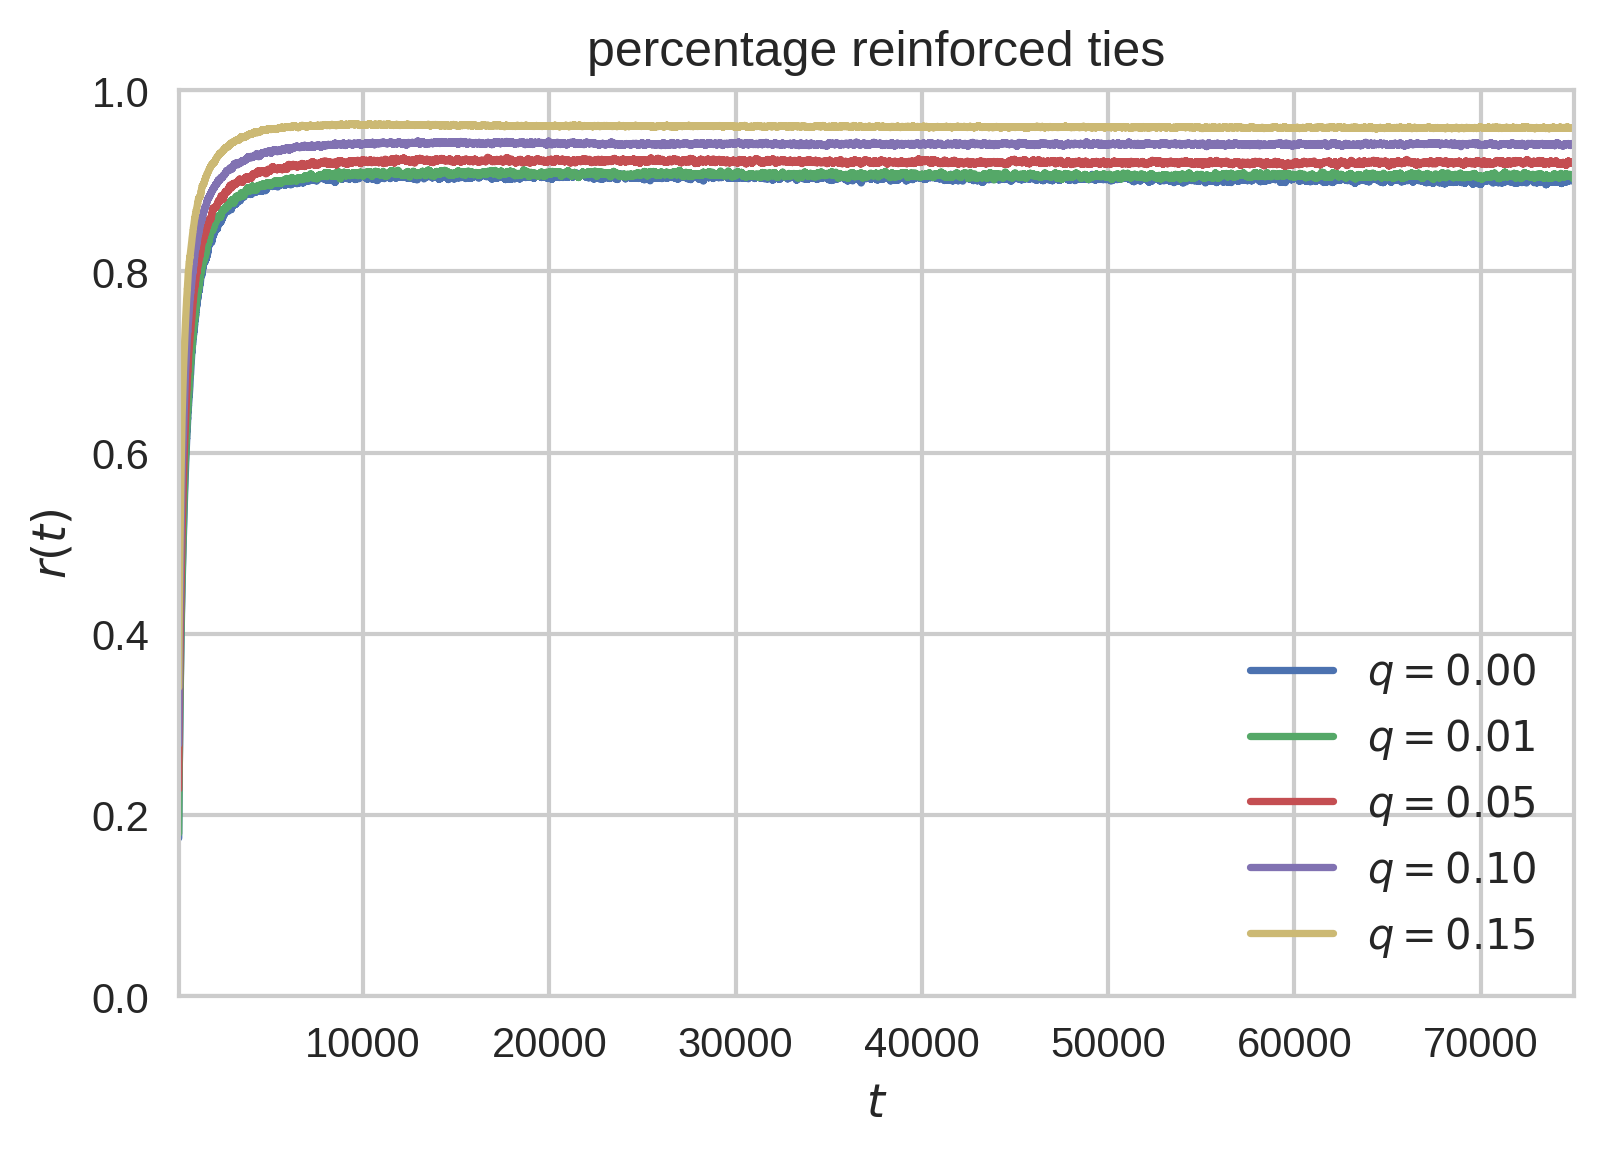
\includegraphics[width=\textwidth]{figures/percentage-reinforced-ties-full}
  \caption{}
  \label{fig:percentage-reinforced-ties-full}
\end{subfigure}
~
\begin{subfigure}[b]{0.485\textwidth}
  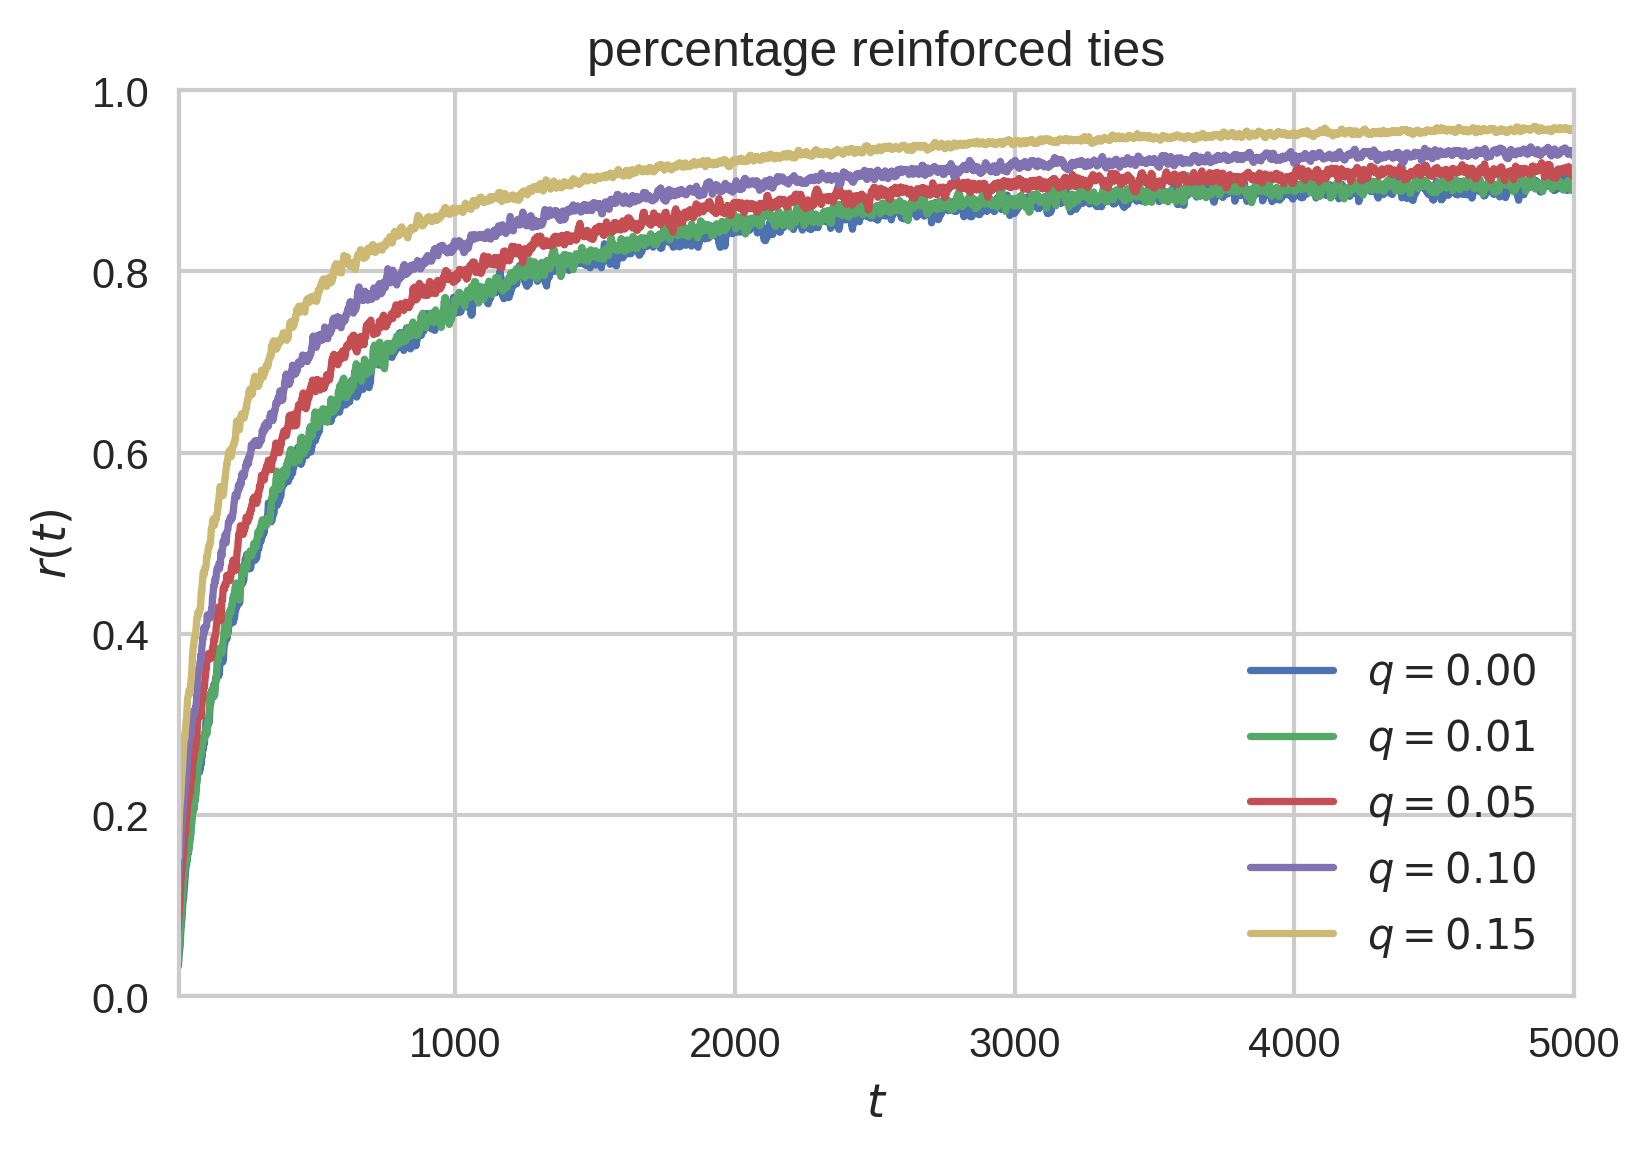
\includegraphics[width=\textwidth]{figures/percentage-reinforced-ties-beginning}
  \caption{}
  \label{fig:percentage-reinforced-ties-beginning}
\end{subfigure}

\caption[Percentage of reinforced ties as function of time]{The percentage of reinforced ties \( r(t) = \sfrac{\#e_{r}(t)}{(\#e_{r}(t) + \#e_{c}(t))} \) for different levels of peer influence as a function of time, where \( \#e_{c}(t) \) and \( \#e_{r}(t) \) are the number of created ties and the number of reinforced ties in iteration \( t \), respectively. (\subref{fig:percentage-reinforced-ties-full}) shows the ratio over all 75,000 iterations and (\subref{fig:percentage-reinforced-ties-beginning}) highlights the behavior in the beginning. Both functions were smoothed using the rolling mean method to improve the quality of the plot.}
\label{fig:percentage-reinforced-ties}
\end{figure}


The evolution of the average local clustering coefficient does dependent on the node deletion probability \( p_{d} \), since low-activity nodes, which are not removed fast enough, introduce additional weak ties in the network~\cite{Laurent2015}.
However, as clearly evident in \cref{fig:avg-local-cc-full}, the possible level of peer influence does influence the clustering, and therefore the community structures of the network, as well.
The more likely an activation due to peer influence gets, the smaller the stationary value for \( C \) becomes.
\Cref{fig:avg-local-cc-end} highlights this effect well.
This can possibly be explained in a similar way as the effect caused by the deletion probability.
However, in this case not the decelerated removal of nodes is responsible for it, but the overall increase in the number of contacts between nodes.
The peer influence mechanism increases the activity in the network, especially in already formed communities (see \cref{sec:network-activity}), since active nodes motivate their neighbors to become active as well.
The probability for the formation of a new tie is inverse proportional to the size of a nodes' egocentric network.
Therefore, a active node, which is already fully integrated in its community, will reinforce one of its existing ties, or at least close a triangle, with high probability.
However, given enough tries, such a node will eventually introduce new weak ties using the focal closure mechanism as well.
Therefore, the opportunities for the introduction of random links by active nodes increases, which leads to a smaller average local clustering in general.

Two additional measures of the integrated network, the average node degree and the average tie strength, were tracked over time for different magnitudes of peer influence as well.
\Cref{fig:avg-weight-and-tie-strength} depicts the graphs for these two network properties as function of time.
Both measures show a similar general behavior.
The average degree and the average tie strength are not independent on the maximum peer influence probability in the network and do converge after the integrated network reaches its equilibrium.
The stationary values of both do increase with increasing values for \( q \) by about the same order of magnitude, which is reasonable since both measures are related to each other.
The tie strength of a node can be seen as its weighted degree.
However, the time it takes until they converge differs.
The average degree takes longer to reach its stationary value.
This can be explained by the small probability for the creation of new ties after the egocentric networks have gained a certain size.
Every new neighbor reduces the probability for the creation of new tie in the future significantly.
The average tie strength does not suffer from this problem, due to the fast development of strong ties and the decreasing probability for the introduction of weak ties. \todo{sound explanation?}
The direct effect of the peer influence mechanism on the average degree and average weight can be explained, similar to the average local clustering coefficient, by the additional activity in the temporal network.
Nodes are getting more opportunities to add additional neighbors and to strengthen their ties until they get removed.
Note that the slightly different convergence behavior of the average tie strength for the high peer influence probability \( q = 0.15 \) cannot be explained fully at this point. It may be related to the by comparison significantly slower converge of the average degree, but it is ultimately left open for possible future studies. \todo{related work}


\begin{figure}[htbp]
\centering
\begin{subfigure}[b]{0.485\textwidth}
  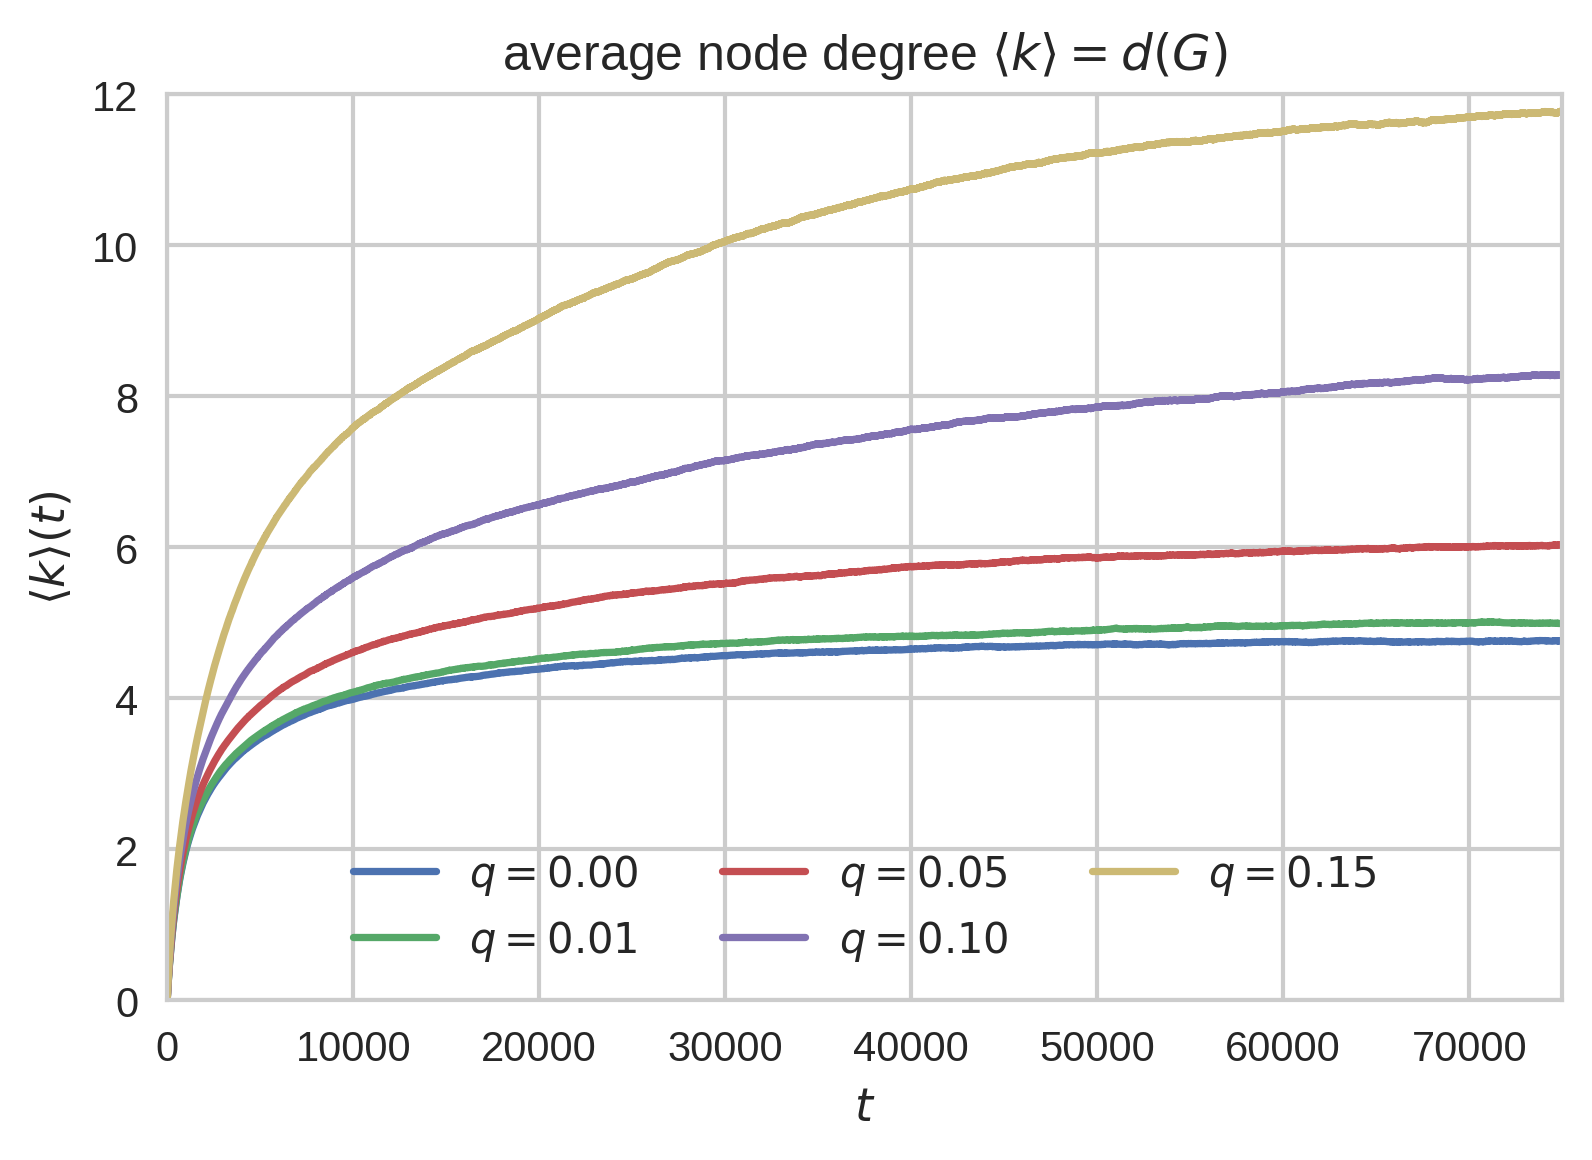
\includegraphics[width=\textwidth]{figures/avg-degree}
  \caption{}
  \label{fig:avg-degree}
\end{subfigure}
~
\begin{subfigure}[b]{0.485\textwidth}
  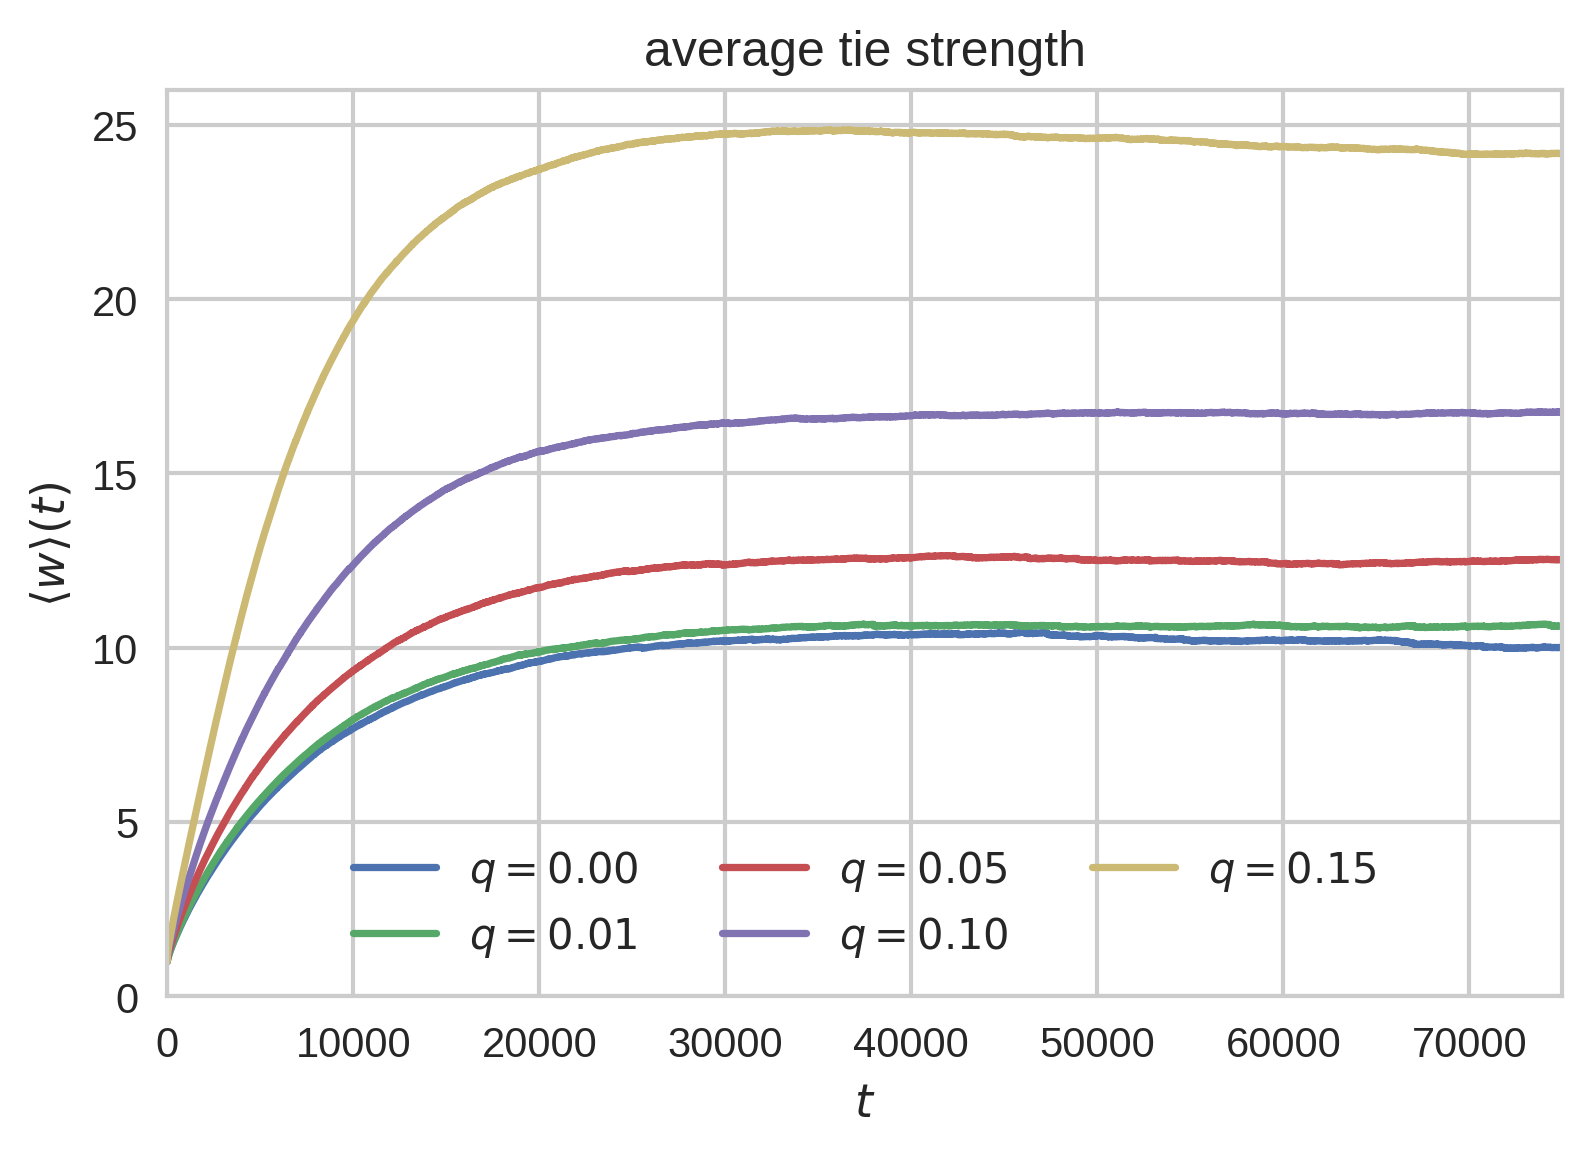
\includegraphics[width=\textwidth]{figures/avg-tie-strength}
  \caption{}
\label{fig:avg-tie-strength}
\end{subfigure}

\caption[Average degree and tie strength as function of time]{Plots of (\subref{fig:avg-degree}) the average node degree \( d(G_{T}) \) and (\subref{fig:avg-tie-strength}) the average tie strength \( \langle w \rangle \) in the network as a function of time for different maximum peer influence probabilities \( q = 0, \, 0.01, \, 0.05, \, 0.1, \, 0.15\). }
\label{fig:avg-weight-and-tie-strength}
\end{figure}


%% ========================================================================
%% ========================================================================


\section{Network Activity}
\label{sec:network-activity}


One obvious implication of the proposed peer influence mechanism is an increase in the activity in the network.
Nodes can become active by them self not only due to their intrinsic activity potential but also by the influence of their peers.
The number of nodes that become active in iteration \( t \) entirely by them self is denoted as \( \#e_{a}(t) \), and the number that becomes active motivated by others is denoted as \( \#e_{p}(t) \).
Therefore, the total number of contacts per iteration is \( \#e(t) = \#e_{a}(t) + \#e_{p}(t) \).
The number of peer influenced activations in a networks with \( q = 0 \) is trivially \( \#e_{p}(t) = 0 \), and the number of self-activations can be approximated by \( \#e_{a}(t) \approx n \expval{a_{i}} \).
For example, the approximated number of activations in a network with no peer influence effects and the prior specified parameters (\( \gamma = 2.7 \), \( \varepsilon = 0.001 \), and \( n = 5,000 \)) is \( \#e_{a}(t) \approx 12.05 \), which matches the observed figures.
In fact, this number is roughly the same for all levels of peer influence, since the process of node self-activation due to the intrinsic activity potential is independent of the peer influence mechanism.


\myfig{number-of-contacts}
      {width=0.75\textwidth}
      {Time dependent number of activations \( \#e(t) \) in the network for different levels of peer influence \( q \). The graphs were smoothed using the rolling mean method to improve the visualization.}
      {Time dependent number of activations}
      {fig:number-of-contacts}


The total number of activations, and therefore the gain in activity due to the peer influence, is depicted in \cref{fig:number-of-contacts}.
It shows that \( \#e(t) \) reaches a stationary value fast for small levels of peer influence.
However, the development of the total number of contacts per iteration is more complex for networks with a higher degree of peer influence.
The first phase can be described as a rapid increase in the number of activations, which stops after approximately 8,000 iterations.
After that the development of \( \#e(t) \) starts to relax and slow down.
It even starts to decreases slightly in the network with a maximum peer influence probability of \( q = 0.15 \).
Finally, the numbers slowly converge to their stationary values, which are reached after about 40,000 iterations.
This is also supported by the evolution of the fraction of the peer influenced contacts per iterations \( i(t) \), which shows the same general behavior (c.f. \cref{fig:percentage-peer-influenced-activity}).
This effect on the total activity in the network is possibly related to the development of the community structures and its implications on the peer influence mechanism.
The stagnation (or even reduction) of the activity begins after the maximum value for the average local clustering coefficient was reached (c.f. \cref{fig:avg-local-cc-full} for details), which is caused by the introduction of weak ties.
These new ties are possibly responsible for the merging of communities in the network, which in turn reduces the effects of the peer influence mechanism.
Inactive nodes in these newly merged communities may have a greater impact on the weighted fraction of active nodes that is required for a significant influence on nodes.
This is could especially be true for weakly integrated nodes.
However, a more detailed analysis has to be performed in the future to determine and verify the true effects, which are responsible for the observed behavior in the network activity for larger magnitudes of peer influence. \todo{future work}


\begin{figure}[htbp]
\centering
\begin{subfigure}[b]{0.485\textwidth}
  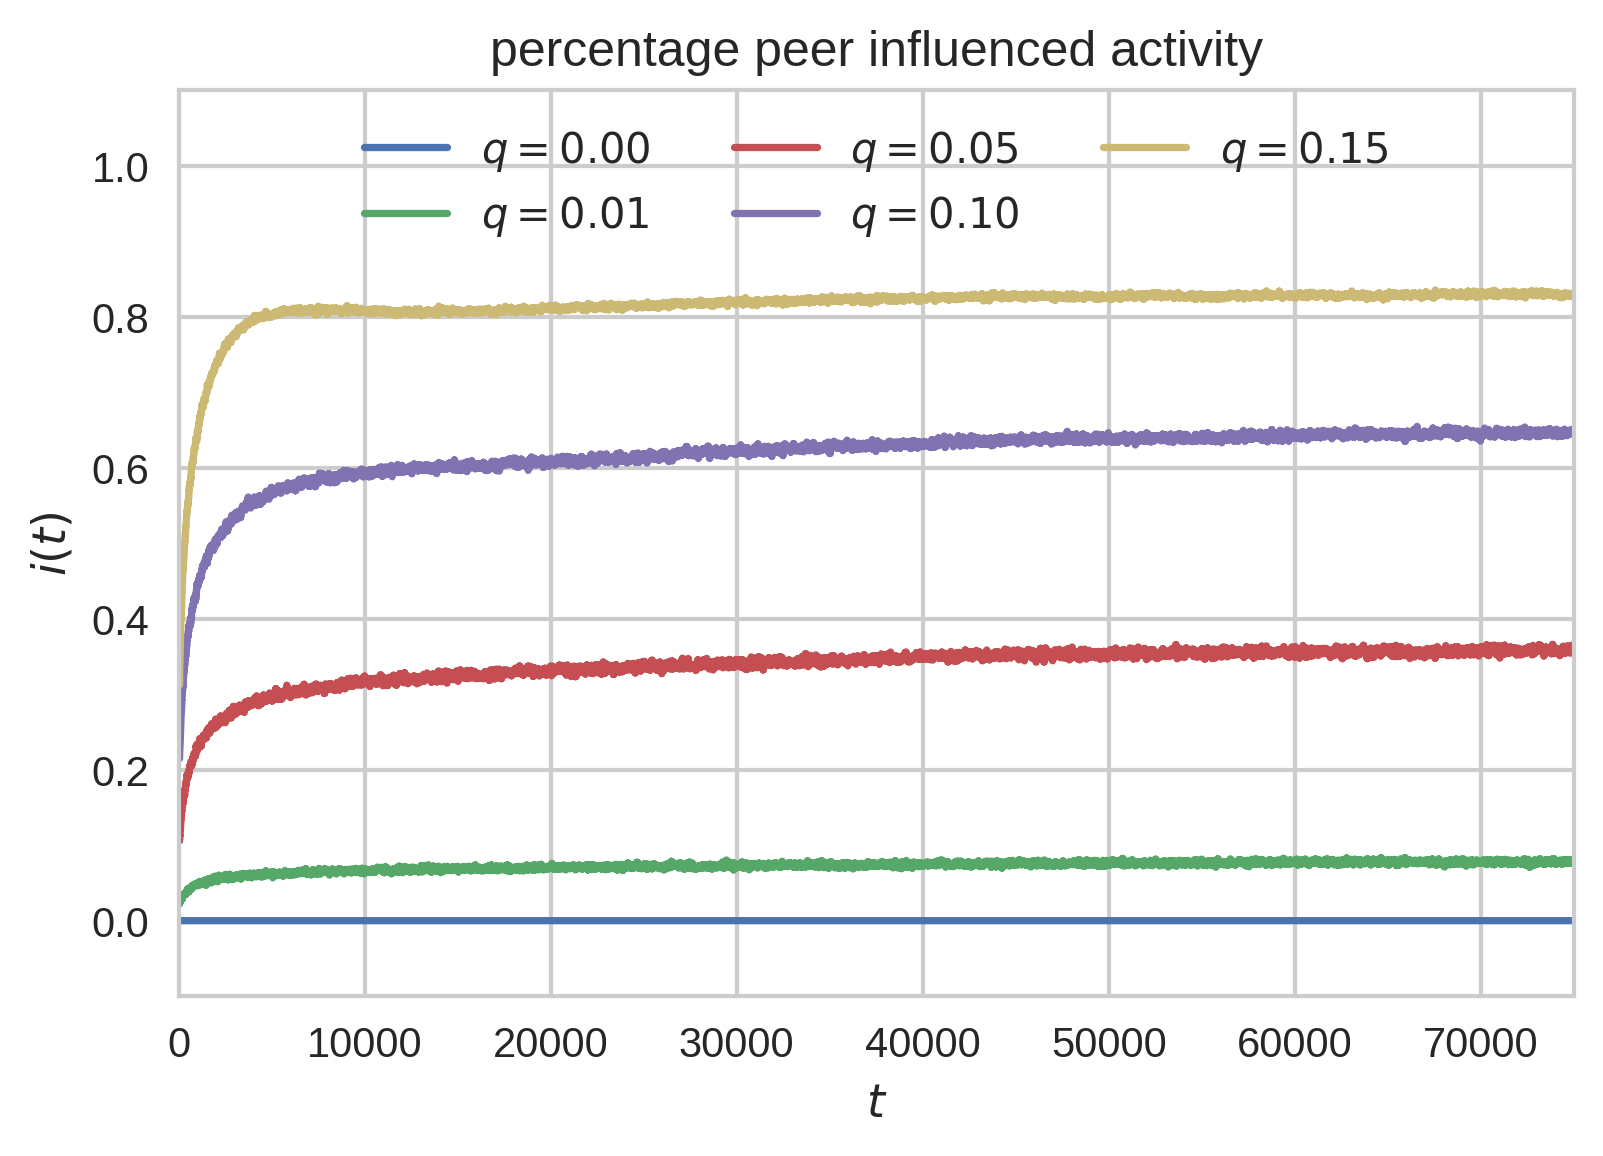
\includegraphics[width=\textwidth]{figures/percentage-influenced-activity}
 \caption{}
 \label{fig:percentage-peer-influenced-activity-full}
\end{subfigure}
~
\begin{subfigure}[b]{0.485\textwidth}
  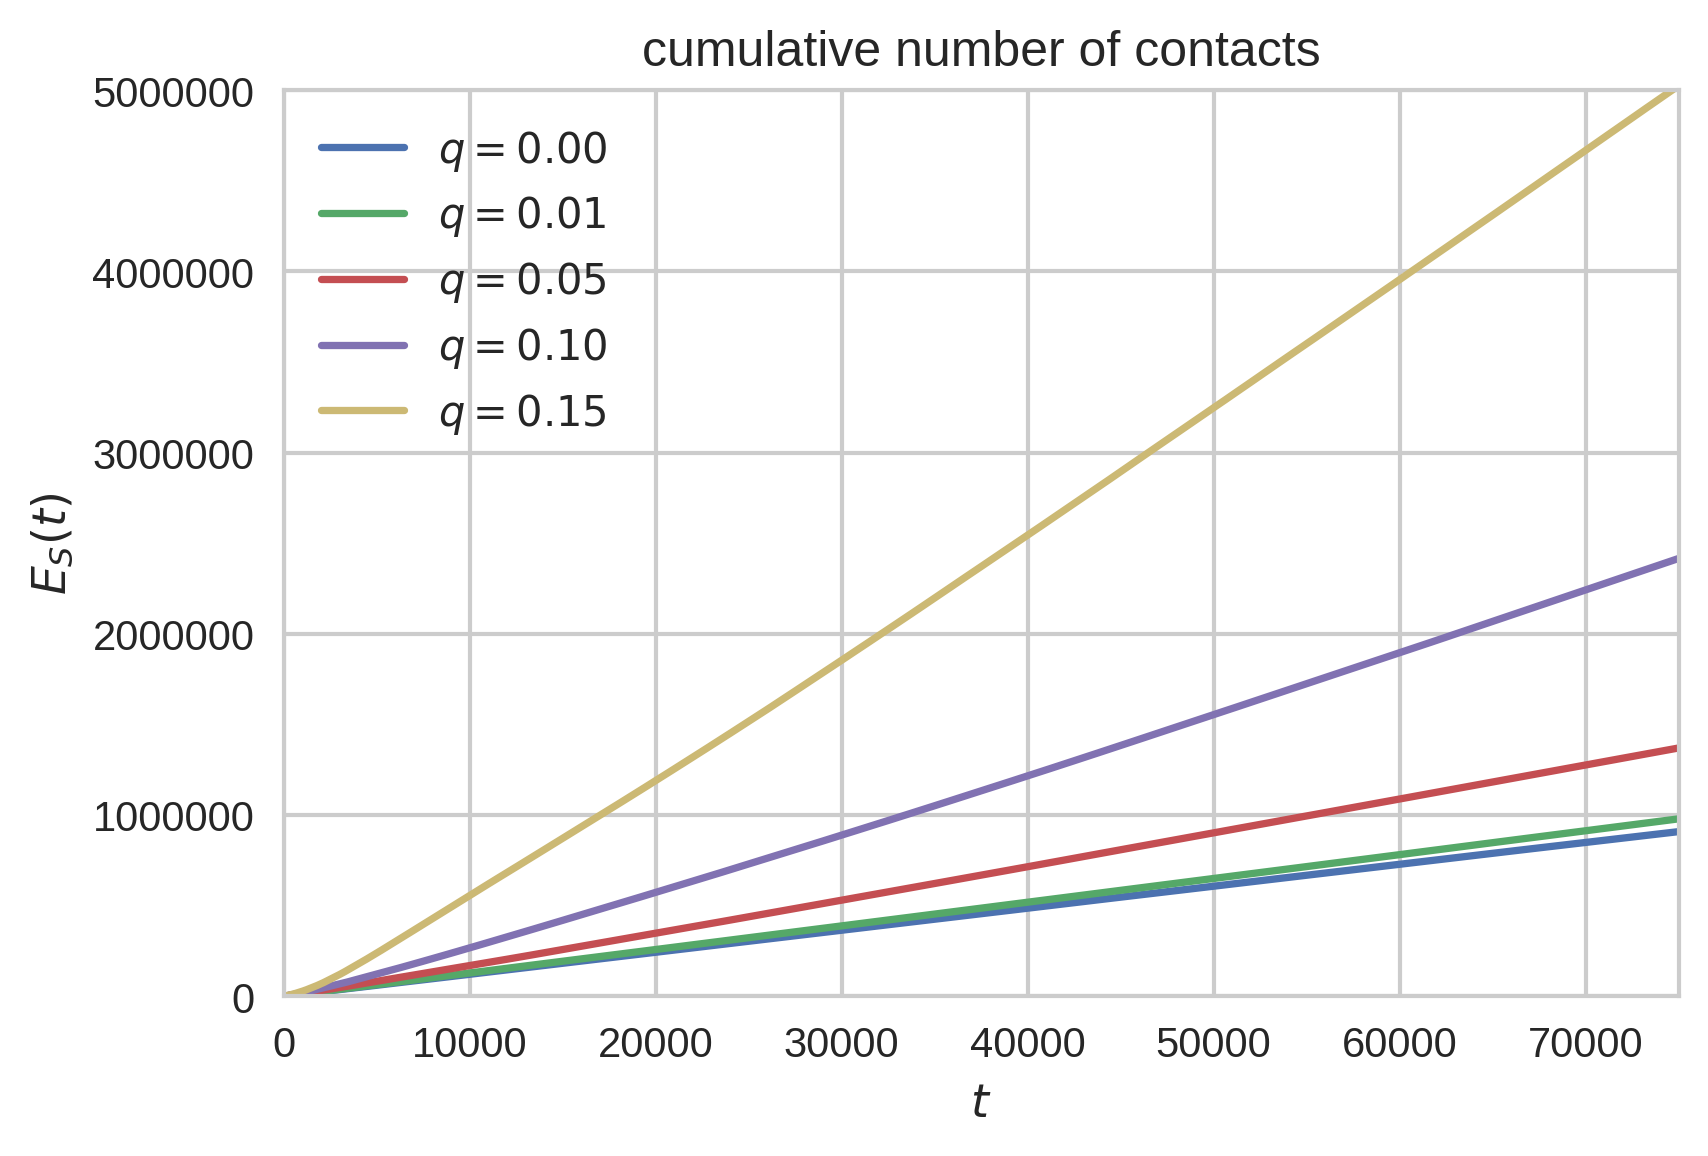
\includegraphics[width=\textwidth]{figures/cumulative-number-of-contacts}
  \caption{}
\label{fig:percentage-peer-influenced-and-cumulative-activity}
\end{subfigure}

\caption[Percentage of peer influenced activity and cumulative activity as function of time]{Different views on the ramifications of the peer influence mechanism on the activity in the network. (\subref{fig:percentage-peer-influenced-activity-full}) depicts the evolution of the fraction of peer influenced activity \( i(t) = \sfrac{\#e_{p}(t)}{\#e(t)} \) over time for different levels of peer influence and  (\subref{fig:percentage-peer-influenced-and-cumulative-activity}) shows the aggregated number of contacts \( E(t) \) over all 75,000 iterations. The \( i(t) \) graphs were smoothed using the rolling mean method to improve the quality of the plot.}
\label{fig:percentage-peer-influenced-activity}
\end{figure}


The effects of the peer influence mechanism on the activity within the time-varying network can be observed in other ways as well.
For instance, \cref{fig:percentage-peer-influenced-and-cumulative-activity} depicts the cumulative number of contacts (i.e., \( E(t) = \sum_{i \leq t} \#e(i) \)), which highlights the quantity of additional activity that was caused by different degrees of peer influence mechanism over time.
The distribution of the number of node activations in a certain time interval is another example.
There is a shift in the bulk of the distributions, which indicates the increased probability for a larger number of activations of a node.


%% ========================================================================
%% ========================================================================


\section{Inter-event Time Distributions}
\label{sec:inter-event-time-dists}

As already mentioned in the motivation section of this thesis (\cref{sec:temporal-data}) and while discussing different ways to model user activity (\cref{sec:user-activity-models}), human activity patterns can be fairly complex.
They can be described as bursts followed by longer phases of inactivity and are usually characterized by the inter-event time distribution \( \varphi(\tau) \), which should reflect these requirements.
The inter-event times are defined, in the context of this model, as the time between two consecutive activations of a node.
The type of activation (i.e., activation due to peer influence, activity potential, or contact of another active node) is not taken into account for the here performed analysis.
Each node \( v_{i} \) in the network has its own inter-event time distribution \( \varphi_{i} \), which depends on the node's activity potential and on the influence of its peers.
However, to get a better overview on how the peer influence mechanism changes the dynamics in the network in general, the union of the inter-event time distributions of all nodes is examined.
The sequence of inter-event times is determined for every node that was active between the beginning and the end of the simulation separately and then combined into one distribution.
This distribution can be seen as a mixture of distributions~\cite{Seidel2011} of nodes, which were at some time present in the network, i.e.,

\begin{equation}
    \varphi(\tau) = \sum_{i} \pi_{i} \varphi_{i}(\tau),
\end{equation}

where \( \pi_{i} \) denotes the mixing weights, which must be selected such that \( \sum_{i} \pi_{i} = 1 \) holds.
Therefore, the mixing weights determine the importance of every individual distribution.
In this work every distribution is considered equally important and is assigned the same weight, such that the summation constraint is fulfilled.

The burstiness of human behavior is difficult to describe and even more difficult to quantify.
It is usually done using moments of the inter-event time distribution.
For instance, the coefficient of variation~\cite{Masuda2016} is defined as the ratio between the standard deviation \( \sigma \) and the mean \( \mu \) of the inter-event time distribution, i.e., \( c_{v} = \sfrac{\sigma}{\mu} \).
It takes the value \( 0 \) when the events are occurring at a fixed non-random rate.
The coefficient of variation is \( 1 \) for exponentially distributed inter-event times, which is the case for events that are generated by a Poisson process, and it can get arbitrarily large for long-tailed distributions, such as power laws.
A normalized variant of the coefficient of variation was proposed by \citet{Goh2008}, which is called burstiness parameter and is defined as

\begin{equation}
    B = \frac{c_{v} - 1}{c_{v} + 1} = \frac{\sigma - \mu}{\sigma + \mu},
\end{equation}

and takes values in the range \( -1 \leq B \leq 1 \).
It is \( B = -1 \) for regularly occurring events, \( B = 0 \) for inter-event times that originated from a Poisson process, and \( B = 1 \) for a distribution that was derived from a extremely bursty sequence of events.
A nice property of this measure is that it can also be applied to mixture distributions that contain the inter-event times of, for example people, with different intrinsic activity levels.
For instance, the inter-event times of power-users that use a system heavily every day can be combined with those of users that use it only irregularly and the burstiness parameter is able to capture the level of burstiness that is present in the usage of the system regardless.
Therefore, it is also applicable for the inter-event time distributions derived from the simulations of the peer influence model.
The burstiness parameter for a network with no peer influence is about \( B = 0.19 \).
The introduction of peer influence increases this value, however, a drastic increase can only be observed for a maximum peer influence probability of \( q \ge 0.15 \).
\Cref{tbl:burstiness-parameter} contains the mean, standard derivation and burstiness parameter of the inter-event time distribution for a maximum peer influence probability in the range \( 0 \leq q \leq 0.15 \).


\begin{table}
\centering
\begin{tabular}{llllllll}
\( q \) & 0.00 & 0.01 & 0.025 & 0.05 & 0.075 & 0.10 & 0.15 \\ \hline
\( \mu \) & 198.71 & 184.59 & 164.26 & 132.80 & 102.43 & 76.28 & 37.23 \\ \hline
\( \sigma \) & 291.32 & 270.49 & 241.40 & 197.38 & 155.09 & 118.04 & 61.22 \\ \hline
\( B \) & 0.1890 & 0.1888 & 0.1902 & 0.1956 & 0.2045 & 0.2149 & 0.2437
\end{tabular}

\caption[Burstiness of inter-event time distributions]{Mean value, standard deviation and the resulting burstiness parameter of the inter-event time distribution for different levels of peer influence.}
\label{tbl:burstiness-parameter}
\end{table}


This indicates that the peer influence mechanism influences the burstiness of the node activations.
In a network with no peer influence are two consecutive self-activations independent of each other.
Therefore, the activations happen at a certain rate that is proportional to the activity potential of a node, which leads to exponentially distributed inter-event times~\cite{Moinet2016}.
This should lead to a burstiness parameter that is close to \( B = 0 \).
However, this is not the case for the inter-event times that were generated with the proposed model even though peer influence was disabled (c.f. \cref{tbl:burstiness-parameter}).
It can be explained by the memory effects in the model, which allow reoccurring interactions within groups of nodes and by the inclusion of passive activations due to other active nodes in the calculation of the inter-event times.
A node with a higher intrinsic activity potential will select a node from its local group with high probability.
Hence, this more active node activates less active nodes regularly, which can lead to a more bursty looking activity pattern for the other nodes and explains (at least partially) the burstiness value of \( B = 0.19 \).
The peer influence mechanism of this model should amplify this effect even further, since it increases the activity within communities.
Furthermore, the activation of nodes possibly triggers cascading activations within the communities, which makes bursts more likely as well.


\myfig{inter-event-time-dist-loglog}
      {width=0.75\textwidth}
      {Log-log Plot of the inter-event time distribution for different maximum peer influence probabilities \( q = 0, \, 0.01, \, 0.05, \, 0.1, \, 0.15\).}
      {Log-log plot of the inter-event time distribution}
      {fig:inter-event-time-dist-loglog}


\myfig{inter-event-time-dist-start}
      {width=0.75\textwidth}
      {Plot of the bulk of the inter-event time distribution for small inter-event times in the range \( 1 \leq \tau \leq 10 \) for different levels of peer influence.}
      {Bulk of the inter-event time distribution}
      {fig:inter-event-time-dist-start}


One way to examine how the peer influence mechanism changes the inter-node-activation times in the network is to inspect their distribution visually.
\Cref{fig:inter-event-time-dist-loglog} depicts the inter-event distributions for a variety of peer influence levels.
The plot shows the distribution on a log-log graph, where both axis are scaled logarithmically.
This highlights that longer inter-event times are indeed possible between two consecutive activations.
The plot also shows that the level of peer influence in the network changes the shape of the distribution.
Smaller inter-event times become more likely for higher levels of peer influence, which can also be seen in the change in the mean of the distributions (c.f. \cref{tbl:burstiness-parameter}).
The average time between activations decreases from about 200 in a network with no peer influence at all, to 38 in a network with \( q = 0.15 \).
The changes in the distribution is even more noticeably for inter-event times less than ten time steps.
\Cref{fig:inter-event-time-dist-start} depicts the distributions for this interval of \( \tau \).
The probability for two successive activations increases drastically from less than 2\% to almost 22\% over the range of possible values for \( q \).
This development of the probabilities possibly explains the increase of the burstiness of the distributions, since a larger number of events within a small time frame becomes more probable due to the peer influence mechanism.
However, the tail of the inter-event time distribution changes for higher levels of peer influence as well.
Large inter-event times become more and more unlikely for larger values of \( q \), and the length of the tail decreases as well.
The values for the standard derivation of the distributions reflect this behavior as well (c.f. \cref{tbl:burstiness-parameter}).
The standard derivation of the inter-event times in the network with high peer influence effects is only about one fifth of the standard derivation in the network without peer effects.
This, of course, prevents longer intervals of inactivity to a certain extend, which is the second crucial requirement for realistic activity patterns.


%% ========================================================================
%% ========================================================================


\section{Degree and Tie Strength Distribution}
\label{sec:weight-and-degree-distribution}

While \cref{sec:integrated-network-properties} examines the average degree and tie strength as a function of time, are the distributions of these two properties the topic of discussion in this section.
Both distributions are obtained from the extended version of the integrated network, which contains all nodes that were present in the last iteration of the simulation.
The degrees and tie strengths of nodes that were deleted in previous iterations are not part of the results.
The ramifications of the closure mechanisms and the memory process on the distributions were already a subject in the original work by \citet{Laurent2015}.
They showed that both the degrees and the tie strengths are heterogeneously distributed.
Furthermore, the shape of the degree distribution is only slightly effected by the triadic closure probability \( p_{\Delta} \) and the tie reinforcement increment \( \delta \).
However, while not being effected by \( p_{\Delta} \), the tie strength distribution does depended on the memory process of the model.
For instance, larger values for \( \delta \) increase the length of the tail.
Nevertheless, a more important issue are the effects on the degree and tie strength distributions by the proposed peer influence mechanism.

First and most important, the peer influence mechanism does not effect the heterogeneous nature of both distributions, which is an often observed property in many real world networks~\cite{Barabasi2002, Karsai2014}.
The resulting possibilities for nodes with higher degree indicate the presence of hubs, which may play, depending on the context, various important roles in networks.
\Cref{fig:degree-dist} depicts the right-skewed degree distributions for networks with different levels of peer influence.
It shows that not only the average degree in the network is directly effected by the peer influence process, but the distribution itself as well.
Nodes with small degrees become less probable, while higher degree nodes become more frequent with the increasing magnitude of peer influence.
However, the tail of the distribution does not seem to be significantly effected by the process.
The change in the shape of the distribution is in line with the already observed increasing average degree and can be explained by the same argument as well.
The boost in node activations caused by the influence of the neighbors leads to more opportunities for the formation of new ties and consequently to larger egocentric networks.


\myfig{degree-distribution}
      {width=0.75\textwidth}
      {Depiction of a degree distribution of the integrated network for different maximum peer influence probabilities \( q = 0, \, 0.01, \, 0.05, \, 0.1, \, 0.15\).}
      {Degree distribution}
      {fig:degree-dist}


\myfig{weights-distribution}
      {width=0.75\textwidth}
      {Log-log plot of the distribution of the tie strengths (i.e., the link weights) in the integrated network for different degrees of peer influence.}
      {Tie strength distribution}
      {fig:weights-dist}

The memory process is primary responsible for the heterogeneous tie strength distribution and the introduction of the peer influence mechanism does in fact not change the distribution in a significant way.
\Cref{fig:weights-dist} shows the distributions for different values for the maximum peer influence probability.
It could be expected that the increased activity within the temporal network would extend the tail of the distribution, however, this is not the case.
A possible explanation of this effect is related to the increased average size of the egocentric networks.
More neighbors imply a larger number of strong ties as well, which require frequent contacts to develop.
Therefore, the additional activations caused by the peer influence mechanism are spend on the development of the additional strong ties and not reinforcing the existing ones, which would enlarge the tail.
This would also explain the more frequent weights in the lower double-digit region, which is a consequence of the on average increased tie strength for networks with peer effects.


%% ========================================================================
%% ========================================================================


\section{Tie Strength Rescaling Scenarios}
\label{sec:softmax-rescaling}

Nodes are only able to influence their peers if they were active in the previous iteration.
The magnitude of influence does depend on the strength of the ties between nodes.
This is based on the idea that the activity of a close friend should be more effective to motivate a person to become active as well than the activities of acquaintances.
The weights (i.e., the strength of the ties) are usually rescaled in such a way that larger weights become even larger to amplify the importance of close neighbors.
This can be archived using the softmax function, which also allows to control the weight rescaling process even more using the inverse temperature parameter \( \beta \).
This free parameter can vary in time as well to allow for different rescaling characteristics depending on the progress of the simulation.
Furthermore, it also allows for various peer influence scenarios, in which nodes get influenced in different extents depending on the situation.
This section highlights the ramification on the peer influence mechanism for the following three different weight rescaling strategies.
Note that the results for the scenarios are obtained from synthetic networks with a fixed maximum peer influence probability of \( q = 0.05 \).
All other model parameter are set to the same values that are used in the other experiments as well.

\myparagraph{\( \beta(t) = \langle w \rangle (t)^{-1} \)}
The temperature for the softmax rescaling is set to the average tie strength in the snapshot of integrated network at time \( t \).
This scenario is used for all other previously discussed experiments in this chapter.
\Cref{sec:integrated-network-properties} shows that the average tie strength does increase over time until it reaches its stationary value.
Therefore, this effectively introduces a bias towards stronger ties in the early stages of the simulation that decays over time.
The activity of close neighbors influences nodes in a larger extent in the beginning, which is possibly beneficial for the formation of the community structures.

\myparagraph{\( \beta(t) = 1 \)}
In this scenario the inverse temperature parameter is fixed to the constant value \( 1 \) for each iteration.
Therefore, the bias towards strong ties is overall more prominent compared to the previous scenario and does not change during the entire simulation.
This may lead to situations in which only a very small number of neighbors do actually influence a node once they become active, since weaker ties with other nodes become so insignificant that they do not exercise considerable influence anymore.
Hence, only one of the highly influential neighbors is possibly enough to influence a node at the maximum possible level.

\myparagraph{\( \beta(t) = 0 \)}
In the last scenario \( \beta \) is fixed to \( 0 \), which basically disables the softmax weight rescaling entirely and assigns each tie the exact same weight.
The strength of the tie between any ordered pair of nodes \( (v_{i}, v_{j}) \) in the network is set to \( w'_{i,j} = \sfrac{1}{|N(v_{i})|} \).
This allows neighbors, which share a weak tie with a node to exercise the same degree of peer influence as strong tied neighbors.
Therefore, an on average larger number of active neighbors may be required to reach the maximum possible magnitude of peer influence for a node.

It seems reasonable to examine the change in the network activity for the three different rescaling scenarios, since most of the explanations for the effects observed in the other experiments are related to it.
\Cref{fig:activity-beta-scenarios} shows the number of interactions between nodes and the fraction of peer influenced interactions as function of time for the three different scenarios.
Compared to the rescaling scenario that adapts to the average tie strength in the network, an overall decrease in the number of interactions is observable in the \( \beta = 1 \) scenario.
This behavior can be attributed to an excessive bias towards strong ties.
Nodes only become active by them self due to their intrinsic activity potential or possibly if one or two of their strong tied neighbors were active in the round before.
This possibly restricts possible cascading activations within groups as well, since weakly tied nodes are node able to propagate activations properly.
The number of contacts and the fraction of those activations that were peer influenced increase rapidly in the first few hundred iterations in the \( \beta = 1 \) scenario and decreases slightly after they reached their maximum value.
This small decrease is not observable in the other two scenarios and can possibly be attributed to the weight heterogeneity that starts to emerge at this point in time in the network, which amplifies the effect.


\begin{figure}[htbp]
\centering
\begin{subfigure}[b]{0.485\textwidth}
  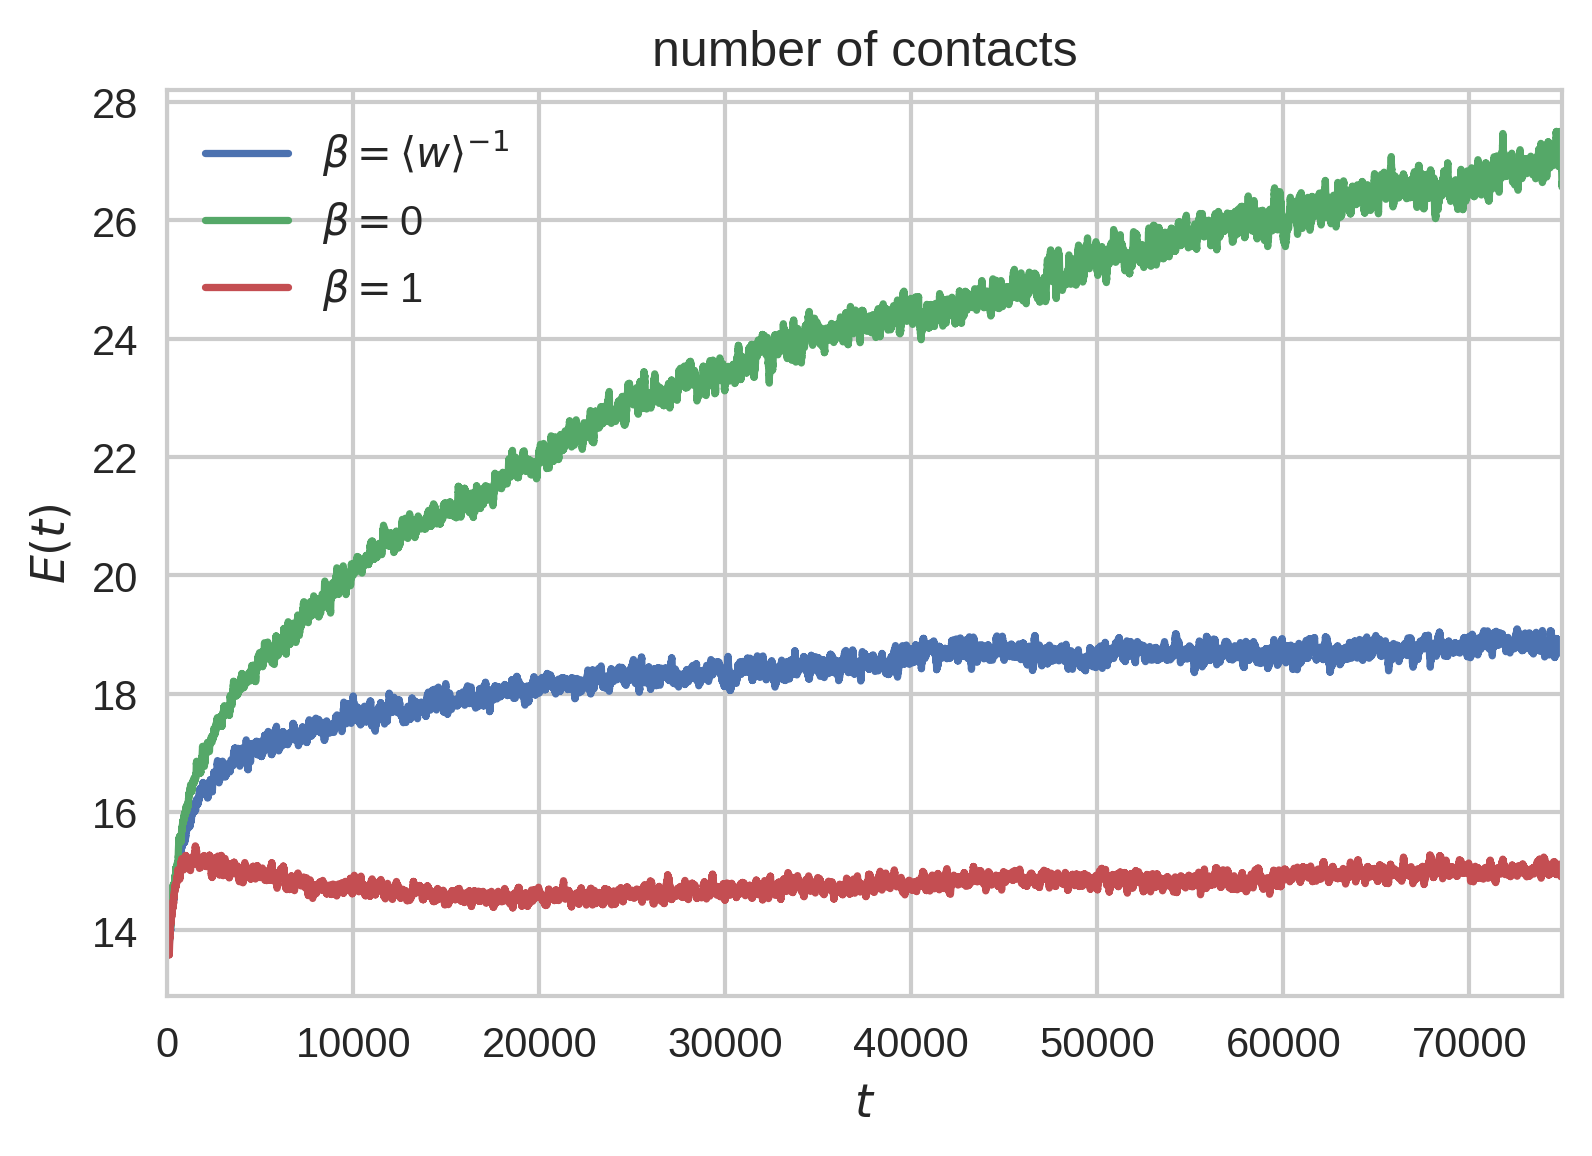
\includegraphics[width=\textwidth]{figures/number-of-contacts-beta}
  \caption{}
  \label{fig:number-of-contacts-beta}
\end{subfigure}
~
\begin{subfigure}[b]{0.485\textwidth}
  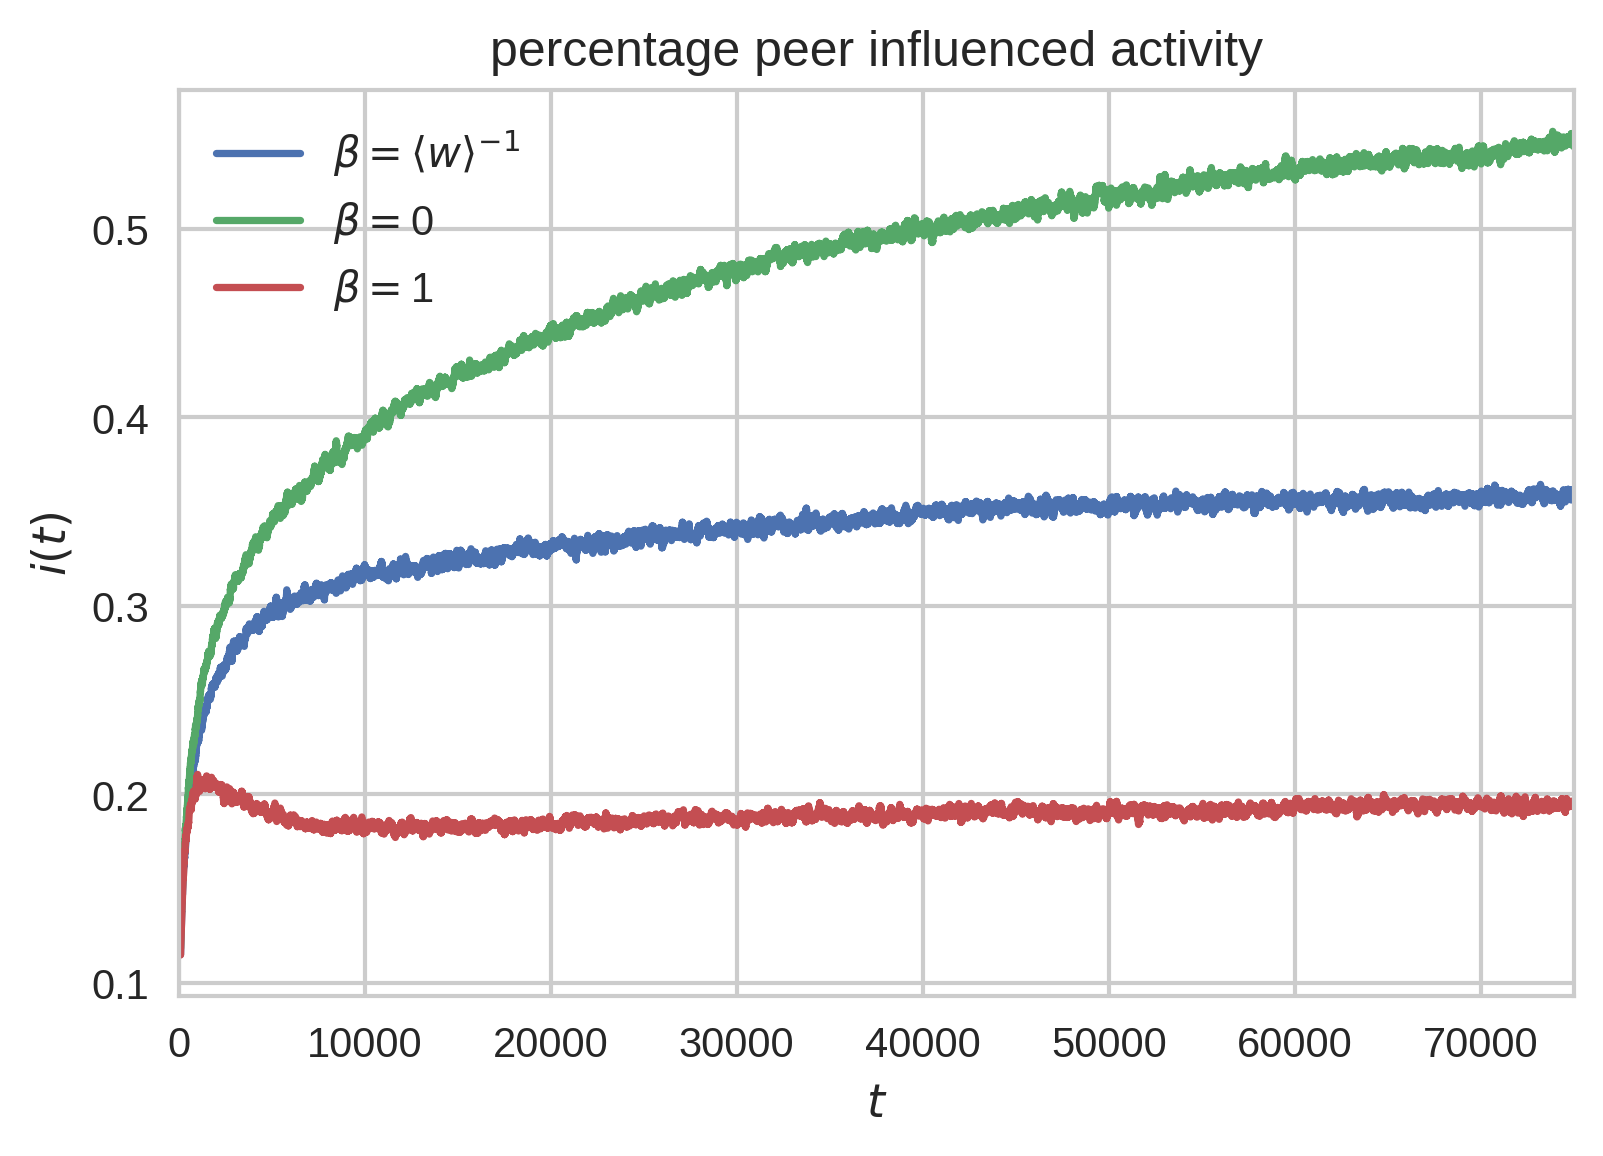
\includegraphics[width=\textwidth]{figures/percentage-influenced-activity-beta}
  \caption{}
\label{fig:percentage-influenced-activity-beta}
\end{subfigure}

\caption[Network activity with different rescaling scenarios]{Depiction of the influence on the activity over time for different values of \( \beta \), the inverse temperature for softmax rescaling. (\subref{fig:number-of-contacts-beta}) shows the number of interactions for each iteration \( \#e(t) \) and (\subref{fig:percentage-influenced-activity-beta}) depicts the fraction of activations that were caused by the peer influence mechanism \( i(t) \). The graphs were smoothed using the rolling mean method to improve the quality of the visualization.}
\label{fig:activity-beta-scenarios}
\end{figure}


The scenario that disables the softmax weight rescaling using \( \beta = 0 \), however, does increase the number of contacts in the network in each iteration drastically.
The expected larger number of active neighbors, which is required to motivate a node seems to be archived fairly often.
This can possibly attributed to the relatively low critical peer influence threshold \( \theta = 0.10 \), which should probably be adjusted for this rescaling scenario.
Furthermore, the network activity does not convergence in this scenario.
One possible explanation for the continuous increase in the number of contacts could be attributed to self-enhancing cascading activation effects going through the network.
However, this requires additional investigation and is a possible topic for future studies. \todo{future work}
